\section{Grupy funkcyjne}
\begin{itemize}
    \item Alkohole
    
    \chemfig[atom sep=2em]{R-OH}
    \newline

    Nazwę związku tworzy się na dwa sposoby. Możemy napisać  "alkohol..." w miejscu kropek wstawiając nazwę związku (łańcucha). Drugim sposobem jest do nazwy łańcucha dodać końcówkę -ol (-3-ol w momencie, gdy grupa hydroksylowa jest dołączona do trzeciego z kolei atomu węgla, itp.).

    \begin{center}
        Przykład:
        
        \chemfig[atom sep=2em]{CH_3-CH(-[6]OH)-CH_3}
        
        alkohol izopropylowy lub propan-2-ol
    \end{center}

    \item Etery
    
    \chemfig[atom sep=2em]{-C-O-C-}
    \newline

    Etery proste, nie zawierające żadnych innych grup funkcyjnych – po słowie eter wymienia się w kolejności alfabetycznej nazwy grup węglowodorowych połączonych z atomem tlenu. Można też etery proste nazywać podstawnikowo, w sposób opisany dla eterów złożonych. Etery symetryczne, w których z atomem tlenu połączone są takie same grupy węglowodorowe, nazywa się podając po słowie eter nazwę grupy węglowodorowej z przedrostkiem –di.

    Etery o bardziej złożonej budowie – nazwę tworzy się jako pochodną macierzystego węglowodoru i dodaje nazwę grupy węglowodorowej przyłączonej do atomu tlenu z końcówką –oksy. Grupę węglowodorową związaną z atomem tlenu traktuje się więc w tym przypadku jak podstawnik w cząsteczce węglowodoru stanowiącego podstawę nazwy.
    \newline

    \begin{center}
    Przykład:

    \chemfig[atom sep=2em]{CH_3-O-CH_2-CH_2-CH_3}
    
    eter metylowo-propylowy lub metoksypropan
\end{center}
    \item Aldehydy
    
    \chemfig[atom sep=2em]{-CHO}

    Nazwę aldehydu tworzy się dodając do nazwy macierzystego alkanu przyrostek –al.

    Niektóre proste aldehydy mają nazwy zwyczajowe, np.: formaldehyd, benzaldehyd.

    \begin{figure}[H]
        \centering
        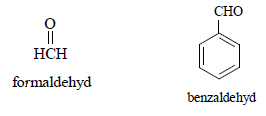
\includegraphics[width=0.5\textwidth]{img/formaldehyd}
        \label{fig.formaldehyd}
    \end{figure}

    \begin{center}
        Przykład:
    
        \chemfig[atom sep=2em]{CH_3-CH_2-CH=[2]O}
        
        propanal
    \end{center}

    \item Ketony
    
    \chemfig[atom sep=2em]{-C=O}

    Nazwę ketonu tworzy się od nazwy macierzystego alkanu dodając przyrostek –on, poprzedzony numerem atomu węgla z grupą karbonylową.

    W przypadku niektórych prostszych związków z tej grupy nazwy tworzy się wymieniając w kolejności alfabetycznej nazwy grup połączonych z grupą karbonylową, poprzedzając je słowem „keton”.

    \begin{figure}[H]
        \centering
        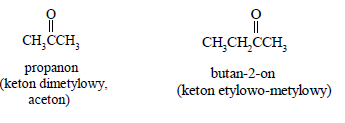
\includegraphics[width=0.7\textwidth]{img/keton}
        \label{fig.keton}
    \end{figure}
    \newpage
    \item Kwasy karboksylowe
    
    \chemfig[atom sep=2em]{-COOH}
    \newline

    Nazwy systematyczne kwasów karboksylowych tworzy się dwojako:
    \begin{enumerate}
        \item Do nazwy macierzystego alkanu z końcówką –owy dodaje się słowo kwas, a atom węgla w grupie karboksylowej jest oznaczany jako C1.
        \item Nazwa łańcucha głównego nie obejmuje grupy karboksylowej, a atom węgla, z którym połączona jest grupa karboksylowa, jest oznaczany jako C1. Do nazwy macierzystego alkanu dodaje się wówczas słowo kwas i końcówkę -karboksylowy.
    \end{enumerate}

    Niektóre związki można też nazwać zwyczajowo:

    \begin{figure}[H]
        \centering
        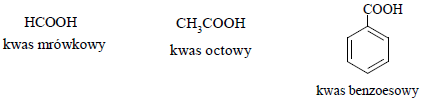
\includegraphics[width=0.7\textwidth]{img/mrówkowy}
        \label{fig.mrówkowy}
    \end{figure}

    \begin{center}
        Przykład:
    
        \chemfig[atom sep=2em]{CH_3-CH_2-COOH}
        
        kwas propanowy lub kwas etanokarboksylowy
    \end{center}

    \item Halogenki kwasowe
    
    \chemfig[atom sep=2em]{R-C(=[2]O)-X}

    Nazwy halogenków kwasowych tworzy się podając nazwę odpowiedniego halogenku i grupy acylowej (systematyczną lub zwyczajową). 

    \begin{center}
        Przykład:
    
        \chemfig[atom sep=2em]{CH_3-C(=[2]O)-Cl}
        
        Chlorek etanoilu

        Chlorek acetylu
    \end{center}

    Związki te można również nazywać w oparciu o nazwę kwasu macierzystego, poprzedzając ją nazwą odpowiedniego halogenku.

    \begin{center}
        Przykład:
    
        \chemfig[atom sep=2em]{CH_3-CH_2-C(=[2]O)-Br}
        
        Bromek kwasu propanowego
    \end{center}

    \item Bezwodniki kwasowy
    
    \chemfig[atom sep=2em]{R-C(=[2]O)-O-C(=[2]O)-R}

    W przypadku bezwodników symetrycznych (otrzymywanych z takiego samego kwasu karboksylowego) nazwy tworzy się, zastępując słowo kwas słowem bezwodnik lub dodając słowo bezwodnik do nazwy macierzystego kwasu.

    \begin{center}
        Przykład:
    
        \chemfig[atom sep=2em]{CH_3-C(=[2]O)-O-C(=[2]O)-CH_3}
        
        Bezwodnik octowy
    \end{center}

    Bezwodniki niesymetryczne (otrzymywane z różnych kwasów karboksylowych) nazywa się podobnie, przy czym nazwy kwasów podaje się w porządku alfabetycznym.

    \begin{center}
        Przykład:
    
        \chemfig[atom sep=2em]{CH_3-C(=[2]O)-O-C(=[2]O)-CH_2-CH_3}
        
        Bezwodnik octowo-propanowy
    \end{center}
    \newpage
    \item Estry
    
    \chemfig[atom sep=2em]{R-C(=[2]O)-O-R'}

    W nazwie estru określa się część kwasową i węglowodorową, najczęściej alkilową (wprowadzoną w miejsce atomu wodoru w grupie karboksylowej). Część kwasowa ma końcówkę –an lub –ian zamiast końcówki –owy występującej w nazwie kwasu macierzystego, część alkilowa (lub inna węglowodorowa) natomiast podawana jest w dopełniaczu.

    \begin{center}
        Przykład:
    
        \chemfig[atom sep=2em]{CH_3-CH_2-C(=[2]O)-O-CH_2-CH_3}
        
        Propanian etylu
    \end{center}

    W przypadku estrów kwasów łańcuchowych zawierających podstawniki w części kwasowej podaje się ich położenie w nazwie, oznaczając atom węgla grupy acylowej numerem 1. Gdy podstawniki znajdują się w części alkilowej (lub ogólnie: węglowodorowej)numeruje się atomy węgla tej części tak, że atom węgla łączący się z atomem tlenu ma numer 1.

    \begin{center}
        Przykład:
    
        \chemfig[atom sep=2em]{CH_3-C(-[2]CH_3)(-[6]CH_3)-CH_2-CH_2-C(=[6]O)-O-CH_3}
        
        4,4-dimetylopentanian metylu
    \end{center}

    \item Amidy
    
    \chemfig[atom sep=2em]{R-C(=[2]O)-NH_2}

    Nazwy amidów tworzy się, dodając do nazwy macierzystego alkanu końcówkę –oamid lub zamieniając końcówkę –yl (-oil) w nazwie grupy acylowej na przyrostek –amid.

    \begin{center}
        Przykłady:
    
        \chemfig[atom sep=2em]{CH_3-C(=[2]O)-NH_2}
        
        Acetamid
    \end{center}
    \begin{center}
         
        \chemfig[atom sep=2em]{CH_3-CH_2-CH_2-C(=[2]O)-NH_2}
        
        Butanoamid
    \end{center}

    Związki te można także określać, poprzedzając nazwę macierzystego kwasu karboksylowego słowem amid.

    \begin{center}
         Przykład:

        \chemfig[atom sep=2em]{CH_3-CH_2-C(=[2]O)-NH_2}
        
        Amid kwasu propanowego
    \end{center}

    W przypadku amidów podstawionych przy atomie azotu najpierw określa się podstawniki, a następnie podaje nazwę amidu macierzystego. Nazwę podstawników poprzedza się lokantem „N”, co oznacza bezpośrednie podstawienie przy atomie azotu.

    \begin{center}
        Przykład:

       \chemfig[atom sep=2em]{CH_3-CH(-[6]Br)-CH_2-C(=[2]O)-N(-[1]H)(-[7]CH_3)}
       
       N-metylo-3-bromobutanoamid
   \end{center}

    \item Nitrozwiązki
    
    \chemfig[atom sep=2em]{-NO_2}

    Do nazwy macierzystego węglowodoru dodaje się przedrostek nitro-. Grupę nitrową traktuje się jako podstawnik, a jej pozycję podaje się wymieniając numer atomu węgla, z którym jest ona związana.

    \begin{center}
        Przykład:

       \chemfig[atom sep=2em]{CH_3CH_2CH_2NO_2}
       
       1-nitropropan
   \end{center}
   \newpage
    \item Aminy
    \begin{enumerate}
        \item pierwszorzędowe
        
        \chemfig[atom sep=2em]{-NH_2}

        Nazwy tworzy się przez dodanie przyrostka –amina do nazwy podstawnika alkilowego. Aminę można potraktować również jako pochodną węglowodoru, zwłaszcza w przypadku amin zawierających inne grupy funkcyjne. Wówczas grupę $-NH_2$ można wymienić jako podstawnik aminowy oraz określić jego pozycję w związku macierzystym.

        \begin{center}
            Przykład:
    
           \chemfig[atom sep=2em]{CH_3CH_2CH_2-CH(-[6]NH_2)-CH_3}
           
           2-aminopentan
       \end{center}

       \begin{center}
        
            \chemfig[atom sep=2em]{CH_3CH_2-CH(-[2]NH_2)-COOH}
       
            kwas 2-aminobutanowy
        \end{center}

        \begin{center}
        
            \chemfig[atom sep=2em]{CH_2CH_2NH_2}
       
            etyloamina
        \end{center}

        \item drugorzędowe
        
        \chemfig[atom sep=2em]{-NH-}

        W przypadku symetrycznych amin do nazwy dodaje się przedrostek di- lub tri-, np.: difenyloamina, trietyloamina.

        \begin{center}
        
            \chemfig[atom sep=2em]{NH(-[2]CH_2CH_3)(-[5]CH_3CH_2)}
       
            dietyloamina
        \end{center}

        Aminy niesymetryczne drugorzędowe i trzeciorzędowe nazywa się jako N-podstawione aminy pierwszorzędowe. Nazwę największej grupy alkilowej wybiera się za nazwę macierzystą, a pozostałe grupy traktuje jako N-podstawniki (dołączone do atomu azotu), wymieniając je w kolejności alfabetycznej.

        \begin{center}
        
            \chemfig[atom sep=2em]{CH_3CH_2CH_2NHCH_3}
       
            N-metylopropyloamina
        \end{center}
        \item trzeciorzędowe
        
        \chemfig[atom sep=2em]{-N(-[6])-}

        \begin{center}
        
            \chemfig[atom sep=2em]{N(-[2]CH_2CH_3)(-[5]CH_3CH_2)(-[7]CH_2CH_3)}
       
            trietyloamina
        \end{center}

        \begin{center}
        
            \chemfig[atom sep=2em]{N(-[3]CH_3CH_2)(-[5]CH_3)-CH_2CH_2CH_2CH_3}
       
            N-etylo-N-metylobutyloamina
        \end{center}
        \item aminy aromatyczne
        \newline

        Aminy aromatyczne traktuje się jako pochodne aniliny (aminobenzenu), a grupy zastępujące atomy wodoru w grupie $NH_2$ aniliny - jako N-podstawniki.

        \begin{figure}[H]
            \centering
            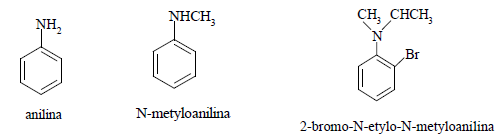
\includegraphics[width=0.7\textwidth]{img/anilina}
            \label{fig.anilina}
        \end{figure}
    \end{enumerate}
    

\end{itemize}
